\section{Results}
\label{sec:results}

\subsection{Inferred velocities}

Figure \ref{fig:results} shows the inferred velocities of 5000 randomly
selected Kepler stars.
The 2D distributions of inferred stellar velocities are plotted in the
lower-left panels, with black contours indicating the stellar number density.
The red contours in these panels show the marginal projections of the
Gaussian prior in 2D.
The diagonal panels show the 1D distributions (histograms) of stellar
velocities.
The black histogram shows the distribution of inferred velocities, the cyan
histogram shows the distribution of velocities calculated for stars with RVs,
and the red lines show the 1D marginal Gaussian prior distributions.
This figure shows that the velocity distributions of stars calculated with and
without RVs are broadly similar.
The prior distribution is calculated using the velocities of stars with RVs.
If the velocity distributions of stars were Gaussian, the 1D red Gaussians
would look like the cyan histograms.
In other words, the differences between the red lines and cyan histograms
is caused by the non-Gaussianity of the velocity distributions.

% Among stars with measured RVs, \vy\ and \vz\ are slightly positively
% correlated: stars with larger \vy\ tend to have larger \vz.
% However, the inferred velocities have the opposite trend: stars with larger
% \vy\ have a smaller \vz.
% This difference is caused by the slight degeneracy between \vy\ and \vz\ for
% stars that do not have RVs.
% The proper motions of stars with a given \vy\ and \vz\ could be equally
% well-described with a slightly larger \vy\ and a smaller \vz\ or vice versa.
% As a result,

\begin{figure}[ht!]
\caption{
The distribution of inferred stellar velocities and distances.
    Figure \ref{fig:results} shows the inferred velocities of 5000 randomly
selected Kepler stars.
The 2D distributions of inferred stellar velocities are plotted in the
lower-left panels, with black contours indicating the stellar number density.
The orange contours in the lower-left panels show the marginal projections of
    the Gaussian prior distribution in 2D.
The upper-right panels in the figure, lying on the plot's diagonal, show the
    1D distributions (histograms) of stellar velocities.
The black histogram shows the distribution of inferred velocities, the blue
histogram shows the distribution of velocities for stars with RVs,
and the orange lines show the 1D marginal Gaussian prior distributions.
}
  \centering
    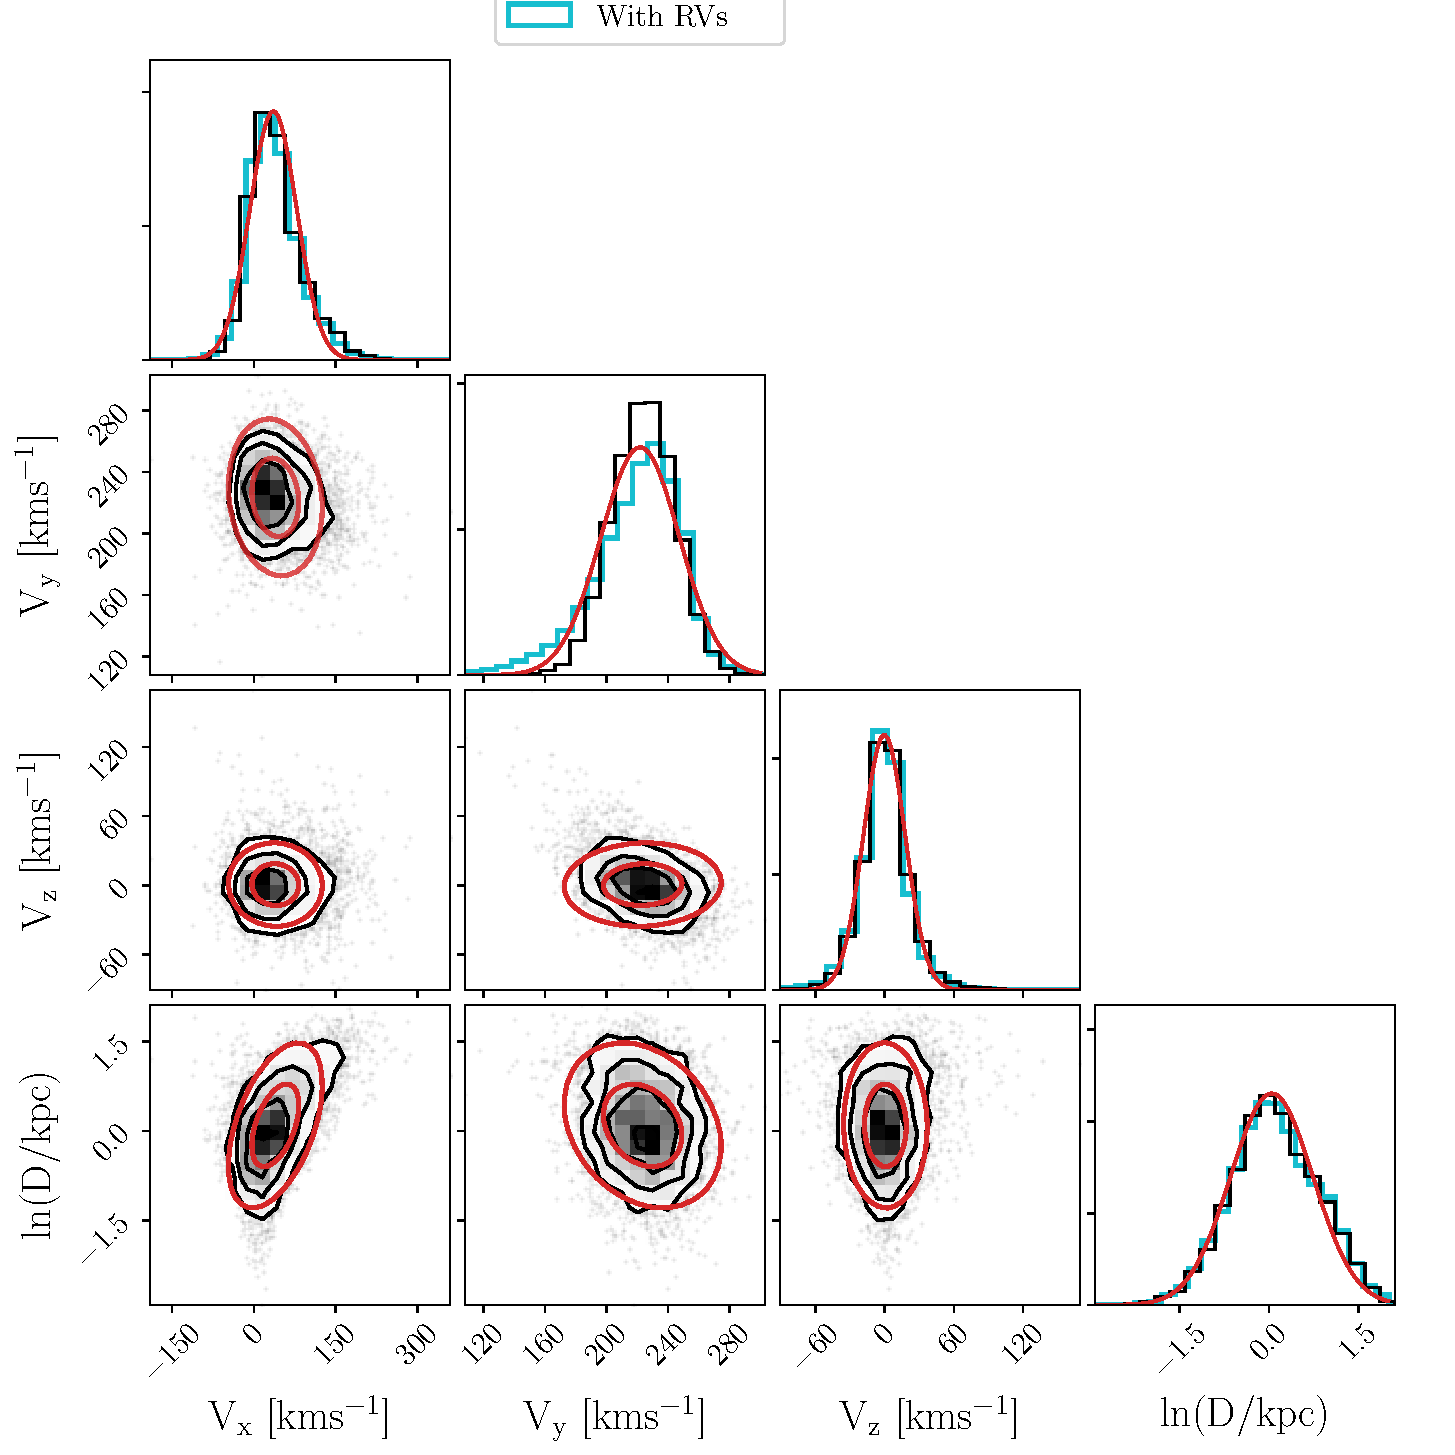
\includegraphics[width=1\textwidth]{results}
\label{fig:results}
\end{figure}


To further validate our method, we compare inferred velocities with
directly-calculated velocities for stars in our sample with measured RVs.
Figure \ref{fig:residuals} shows the \vx, \vy\ and \vz\ velocities, and
distances we inferred, compared with those calculated from measured RVs, for
3000 Kepler stars chosen at random.
\begin{figure}[ht!]
\caption{Velocities calculated with full 6D information compared with
    velocities inferred without RVs, for 3000 Kepler targets with RV
    measurements.}
  \centering
    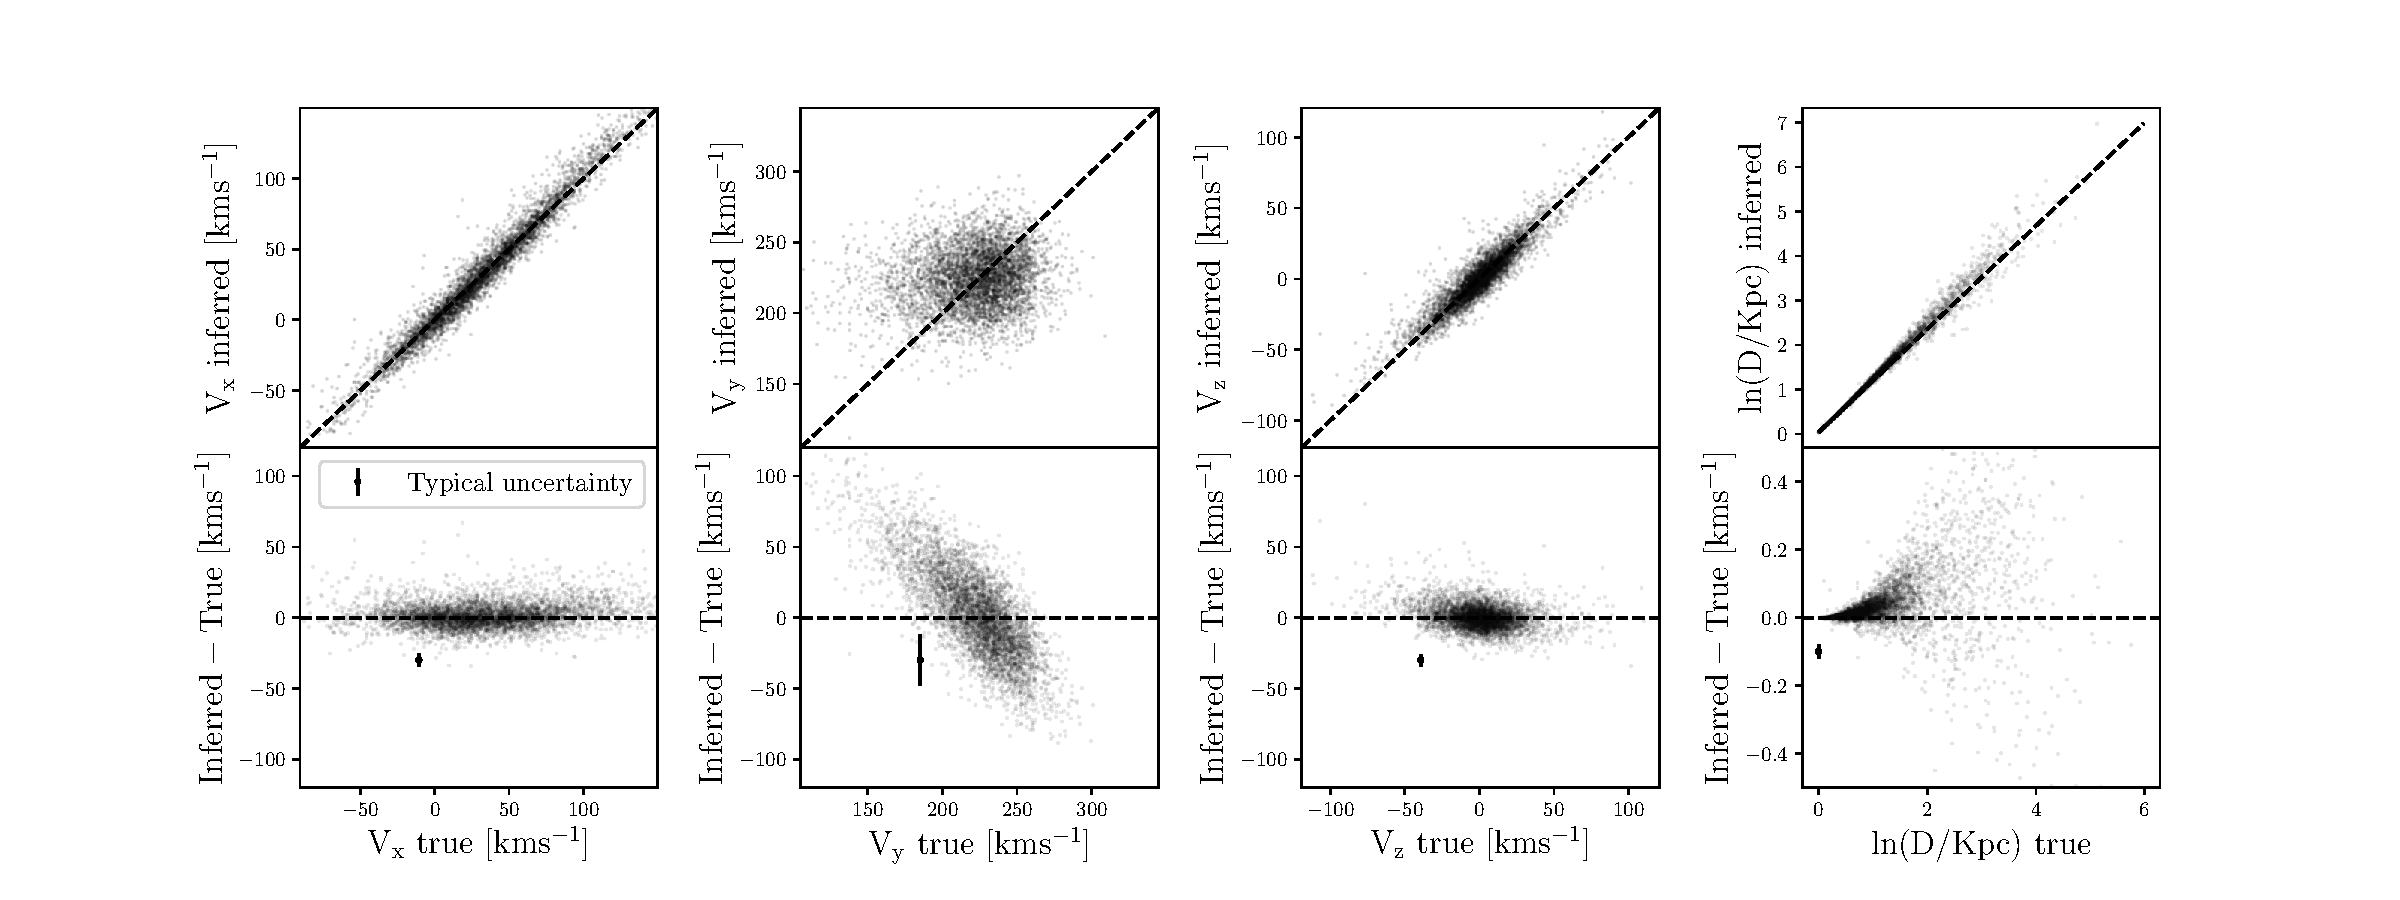
\includegraphics[width=1\textwidth]{residuals}
\label{fig:residuals}
\end{figure}

The three velocity components, \vx, \vy\ and \vz\ were recovered with
differing levels of precision: \vx\ and \vz\ are inferred more precisely than
\vy.
This is because of the position of the \kepler\ field, shown in figure
\ref{fig:kepler_field}.
The velocities of low-\vy\ stars are underestimated and the velocities of
high-\vy\ stars are overestimated.
This is because there is little information to constrain the \vy\ velocities
and the prior pulls the \vy\ velocities toward the center of the distribution.
Velocities in the \y\ and \z\ directions are tightly correlated for Kepler
stars because of the position of the field on the sky.
This means that stars with underestimated \vy\ velocities also have
underestimated \vz\ velocities.
To a lesser degree, \vy\ and \vx\ are correlated too, so underestimated \vy\
also results in a slightly underestimated \vx.

Table \ref{velocity_table} contains the inferred 3D velocities of stars in our
sample, in addition to their positional and velocity information from
Gaia EDR3, LAMOST DR5 and APOGEE DR16.
A sample of this table is displayed here, and the full machine-readable table
is available online.

\ref{tab:data}.
\begin{table}[h!]
  \begin{center}
      \caption{
The velocities calculated in this project (the full table is available
      online).
      }
    \label{tab:data}
\begin{tabular}{cccccc}
    KIC ID & DR3 source ID & $\alpha (^\circ)$ & $\delta (^\circ)$ & $\omega$
    [mas] & Distance [kpc] \\
\hline
1164102 & 0.63 & 4053 & 31.5 $\pm$ 0.5 & 13.6 $\pm$ 0.2 & 21.2 $\pm$ 0.4 \\
1292688 & 0.52 & 3752 & 42.7 $\pm$ 2.1 & -14.2 $\pm$ 0.2 & 21.9 $\pm$ 0.7 \\
1297303 & 0.67 & 4318 & 27.3 $\pm$ 0.2 & 16.7 $\pm$ 0.3 & 16.7 $\pm$ 0.2 \\
1429921 & 0.65 & 4258 & 23.1 $\pm$ 0.1 & -7.0 $\pm$ 0.2 & 14.8 $\pm$ 0.2 \\
1430349 & 0.65 & 4368 & 34.7 $\pm$ 0.8 & 12.2 $\pm$ 0.2 & 19.7 $\pm$ 0.4 \\
1430893 & 0.61 & 3985 & 17.0 $\pm$ 0.0 & 0.4 $\pm$ 0.1 & 9.2 $\pm$ 0.1 \\
1431116 & 0.72 & 4415 & 38.8 $\pm$ 1.0 & -16.5 $\pm$ 0.1 & 19.7 $\pm$ 0.4 \\
1432745 & 0.7 & 4413 & 22.2 $\pm$ 0.2 & -2.1 $\pm$ 0.0 & 13.4 $\pm$ 0.2 \\
1435229 & 0.57 & 4080 & 23.5 $\pm$ 0.0 & -8.8 $\pm$ 1.0 & 13.2 $\pm$ 0.2 \\
1569682 & 0.57 & 3909 & 17.4 $\pm$ 0.2 & 4.4 $\pm$ 0.1 & 9.2 $\pm$ 0.1 \\
\end{tabular}
\end{center}
\tablecomments{This table is published in its entirety in a machine-readable format.
      A portion is shown here for guidance regarding its form and content.}
\end{table}

